\documentclass[crop=false, class=memoir]{standalone}
\usepackage[utf8]{inputenc}%Nødvendig for danske bogstaver
\usepackage[danish]{babel}%Sørger for at ting LaTeX gør automatisk er på dansk
\usepackage{csquotes}
\usepackage{geometry}%Til opsætning af siden
\geometry{lmargin = 2.5cm,rmargin = 2.5cm}%sætter begge magner
\usepackage{lipsum}%Fyldtekst, til brug under test af layoutet
\usepackage{float}
\usepackage{graphicx}%Tillader grafik
\usepackage{epstopdf}%Tillader eps filer
\usepackage{marginnote}% Noter i margen
\interfootnotelinepenalty=10000 %undgår at fodnoter bliver spilittet op.
\usepackage[sorting=none]{biblatex}
\addbibresource{litteratur.bib}
\usepackage[hidelinks]{hyperref}%Tillader links
\usepackage{subcaption} % Tillader underfigurer
\usepackage[font={small,sl}]{caption}	% Caption med skrå tekst ikke kursiv

\usepackage{xcolor} %Bruges til farver
\usepackage{forloop} %Bruges til nemmere for loops

\newcounter{opgave}[chapter] %Definerer opgavenumrene og hvornår de nulstilles
\renewcommand{\theopgave}{\thechapter.\arabic{opgave}} %Definerer udseende af opgavenummereringen
\newcounter{delopgave}[opgave] %Definerer delopgavenumrene
\newcounter{lvl} %Definerer en "variabel" til senere brug

\definecolor{markerColor}{rgb}{0.0745098039, 0.262745098, 0.584313725} %Definerer farven af markøren
\newcommand{\markerSymbol}{\ensuremath{\bullet}} %Definerer tegnet for markøren
\newlength{\markerLength} %Definerer en ny længde
\settowidth{\markerLength}{\markerSymbol} %Sætter den nye længde til bredden af markøren

\newenvironment{opgave}[2][0]{%Definerer det nye enviroment, hvor sværhedsgraden er den første parameter med en default på 0
\newcommand{\opg}{\refstepcounter{delopgave}\par\vspace{0.1cm}\noindent\textbf{\thedelopgave)\space}}%Definerer kommando til delopgave
\refstepcounter{opgave}%Forøger opgavenummer med 1 og gør den mulig at referere til
\setcounter{lvl}{#1}%Sætter "variablen" lvl lig med angivelsen af sværhedsgraden
\noindent\hspace*{-0.75em}\hspace*{-\value{lvl}\markerLength}\forloop{lvl}{0}{\value{lvl}<#1}{{\color{markerColor}\markerSymbol}}\hspace*{0.75em}%Sætter et antal af markører svarende til sværhedsgraden
\textbf{Opgave \theopgave : #2}\newline\nopagebreak\ignorespaces}{\bigskip} %Angiver udseende af titlen på opgaverne samt mellemrummet mellem opgaver



\usepackage{mathtools}%Værktøjer til at skrive ligninger
\renewcommand{\phi}{\varphi}%Vi bruger varphi
\renewcommand{\epsilon}{\varepsilon}%Vi bruger varepsilon
\usepackage{physics}%En samling matematikmakroer til brug i fysiske ligninger
\usepackage{braket}%Simplere kommandoer til bra-ket-notation
\usepackage{siunitx}%Pakke der håndterer SI enheder godt
\DeclareSIUnit\clight{\text{\ensuremath{c}}} % Lysets fart i vakuum som c og ikke c_0
\usepackage{chemmacros}
\usechemmodule{isotopes}
\usepackage{tikz}
\usepackage[danish]{cleveref}
\usepackage{nicefrac}
% \renewcommand{\ref}[1]{\cref{#1}}
\creflabelformat{equation}{#2(#1)#3}
\crefrangelabelformat{equation}{#3(#1)#4 to #5(#2)#6}
\crefname{equation}{ligning}{ligningerne}
\Crefname{equation}{Ligning}{Ligningerne}
\crefname{section}{afsnit}{afsnitene}
\Crefname{section}{Afsnit}{Afsnitene}
\crefname{figure}{figur}{figurene}
\Crefname{figure}{Figur}{Figurene}
\crefname{table}{tabel}{tabellerne}
\Crefname{table}{Tabel}{Tabellerne}
\crefname{opgave}{opgave}{opgaverne}
\Crefname{opgave}{Opgave}{Opgaverne}
\crefname{delopgave}{delopgave}{delopgaverne}
\Crefname{delopgave}{Delopgave}{Delopgaverne}

\newcommand{\eqbox}[1]{\begin{empheq}[box=\fbox]{align}
	\begin{split}
	#1
	\end{split}
\end{empheq}}

\newcommand{\kb}{\ensuremath{k_\textsc{b}}}

\DeclareSIUnit{\parsec}{pc}
\DeclareSIUnit{\lightyear}{ly}
\DeclareSIUnit{\astronomicalunit}{AU}
\DeclareSIUnit{\year}{yr}
\DeclareSIUnit{\solarmass}{M_\odot}
\DeclareSIUnit{\solarradius}{R_\odot}
\DeclareSIUnit{\solarluminosity}{L_\odot}
\DeclareSIUnit{\solartemperature}{T_\odot}
\DeclareSIUnit{\earthmass}{M_\oplus}
\DeclareSIUnit{\earthradius}{R_\oplus}
\DeclareSIUnit{\jupitermass}{M_J}

% Infobokse og lignende
% http://mirrors.dotsrc.org/ctan/graphics/awesomebox/awesomebox.pdf
% \usepackage{awesomebox}


% Egen infobokse (virker kun med begrænsede symboler)

\usepackage[framemethod=tikz]{mdframed}
\usetikzlibrary{calc}
\usepackage{kantlipsum}

\usepackage[tikz]{bclogo}

\tikzset{
    % lampsymbol/.style={scale=2,overlay}
    % lampsymbol/.pic={\centering\tikz[scale=5]\node[scale=10,rotate=30]{\bclampe}}.style={scale=2,overlay}
    infosymbol/.style={scale=2,overlay}
}

\newmdenv[
    hidealllines=true,
    nobreak,
    middlelinewidth=.8pt,
    backgroundcolor=blue!10,
    frametitlefont=\bfseries,
    leftmargin=.3cm, rightmargin=.3cm, innerleftmargin=2cm,
    roundcorner=5pt,
    % skipabove=\topsep,skipbelow=\topsep,
    singleextra={\path let \p1=(P), \p2=(O) in ($(\x2,0)+0.92*(1.1,\y1)$) node[infosymbol] {\bcinfo};},
    % singleextra={\path let \p1=(P), \p2=(O) in ($(\x2,0)+0.5*(2,\y1)$) node[infosymbol] {\bcinfo};},
]{info}

% Skal bruges som
% \begin{info}[frametitle={Titel}]
%     Tekst
% \end{info}
\usepackage{import}
\begin{document}
\chapter{Analytisk Mekanik} \label{chap:mek_opg}

\section*{Koordinatsystemer}
\begin{opgave}[1]{Gode koordinatsystemer}
At få valgt et smart koordinatsystem er essentielt i analytisk mekanik.
%
\opg Beskriv hvad der kendetegner et smart valg af koordinatsystem?
%
\opg Beskriv med egne ord, hvorfor polære koordinater er bedre til at beskrive pendulet end kartesiske koordinater.
% \opg Hvorfor kan det smarte koordinatsystem identificeres ud fra symmetri?
%
% \opg Hvilket koordinatsystem er smartes for et problem med: \\
% a) Plansymmetri. \\
% b) Cylindrisk symmetri. \\
% c) Sfærisk symmetri. \\
% Forklar hvorfor?
\end{opgave}


\begin{opgave}[1]{Generaliserede koordinater}
Betragt et objekt der er fanget på en ring med centrum i origo, $(0,0)$, og radius $R$. \textit{Hint}: se \cref{k-mat:sec:trig} i kompendiet.
%
\opg Definer et sæt polære koordinater $(r,\phi)$, og skriv de kartesiske koordinater op med disse.
%
\opg Hvor mange af de kartesiske koordinater ændres, når objektet bevæger sig på ringen?
%
\opg Hvor mange af de polære koordinater ændres, når objektet bevæger sig på ringen?
%
\opg Hvor mange koordinater skal der bruges for at beskrive objektets bevægelse?
%
\opg Hvad er det smarte koordinatvalg?
%
\end{opgave}


% \begin{opgave}[3]{Brint}
% Hydrogenisotopen $^1$H består af en proton med massen $m_p$ og ladningen $Q = e$ (elementarladningen), samt en elektron med massen $m_e$ og ladningen $q = -e$. Fra elektrostatik\footnote{Elektrostatik er studiet af elektriske felter dannet af stillestående (statiske) elektriske ladninger. For mere information se \cref{k-chap:elektro} i kompendiet.} oplyses det, at kraften fra en punktladning $Q$ med stedvektor $\va{r}_1$ på en punktladning $q$ med stedvektor $\va{r}_2$ er
% %
% \begin{align} \label{mek:eq:F_el}
% 	\va{F} = \frac{qQ}{4\pi\epsilon_0} \frac{\va{r}_2-\va{r}_1}{|\va{r}_2-\va{r}_1|^3},
% \end{align}
% %
% hvor $\epsilon_0$ er en konstant, der kaldes vakuumpermittiviteten. Punktladninger er ladninger uden udstrækning, hvorfor de eksisterer i ét punkt i rummet og kun det punkt. Elektroner og protoner er så små, at det giver god mening at beskrive dem som punktladninger, hvorfor \cref{mek:eq:F_el} kan benyttes.
% %
% \opg Skitser situationen og indtegn systemets massemidtpunkt. \textit{Hint}: Se \cref{mek:eq:CM} for definitionen af massemidtpunktet (engelsk: ``center of mass'', forkortes CM).
% %
% \opg Hvad betyder $|\va{r}_2-\va{r}_1|$ fysisk?
% %
% \opg Indtegn kræfterne på begge ladninger i jeres tegning.
% %
% \opg Hvor er det smartest at placere origo? \\ \\
% %
% Massemidtpunktet for et tolegemesystem er defineret som
% %
% \begin{align} \label{mek:eq:CM}
% 	\va{r}_\textsc{cm} = \frac{m_1\va{r}_1 + m_2\va{r}_2}{m_1 + m_2} \, .
% \end{align}
% %
% \opg Hvad bliver $\va{r}_{\textsc{cm}}$ for vores system under approksimationen at $m_p \gg m_e$?
% %
% \opg Opskriv kraften på elektronen i dette koordinatsystem.
% \end{opgave}


\section*{Approksimation til harmonisk oscillator}

% \begin{opgave}[1]{Energibevarelse} \label{mek:opg:Energibevarelse}%
% Energi er altid bevaret. Den kan omdannes imellem forskellige former, men den forsvinder aldrig.
% %
% \opg Opskriv nogle af de typer af energi, som du kan komme på.
% %
% \opg Forklar i egne ord hvad en konservativ kraft er.
% %
% \opg Summen af kinetisk og potentiel energi kaldes mekanisk energi, og er bevaret i et system, så længe det kun er påvirket af konservative kræfter. Angiv tre eksempler på systemer, hvor den mekanisk energi er bevaret, og tre hvor den ikke er.
% %
% \opg Angiv for hvert eksempel hvor den mekaniske energi ikke er bevaret, hvad årsagen er til dette.
% \end{opgave}


% \begin{opgave}[2]{Frit fald} \label{mek:opg:FritFald}%
% Et legeme med massen $m$ frigives fra hvile i en afstand $h$ over Jordens overflade. Antag at tyngdeaccelerationen er konstant og har værdien $g$.
% %
% \opg Tegn et kraftdiagram for systemet.
% %
% \opg Hvorfor er den mekaniske energi ikke bevaret?
% %
% \opg Negliger nu den kraft der ødelægger energibevarelsen, og bestem legemets fart i det øjeblik det rammer Jorden.
% %
% \opg Diskuter hvor god en antagelse det er, at negligere den ``problematiske'' kraft, og opstil et muligt kriterie for, at det er en god antagelse negligere denne.
% \end{opgave}


% Denne opgave er lidt afkoblet fra resten det gennemgået materiale og udelades derfor.
% \begin{opgave}[1]{Kollisioner}
% Når to legemer kolliderer kan det inddeles i to grupper: elastiske og uelastiske kollisioner. Under kollisionen påvirker legemerne hinanden med en eller flere kræfter, og elastiske kollisioner defineres som kollisioner, hvor disse kræfter udelukkende er konservative. Der ses bort fra eventuelle ydre kræfter.
% \opg Hvorfor er størrelsen af den samlede kraft fra legeme 1 på legeme 2, den samme som den samlede kraft fra legeme 2 på legeme 1?
% \opg I hvilken retning går kraften på legeme 2 i forhold til kraften på legeme 1?
% \opg Benyt Newtons anden lov til at vise, at systemets totale impuls er bevaret.
% \opg Er den kinetiske energi bevaret for en \\
% a) Elastisk kollision? \\
% b) Uelastisk kollision?\\
% \end{opgave}


\begin{opgave}[3]{Bevægelse omkring ligevægt} \label{mek:opg:equilibrium}%
Det antages, at en masse $m$ er påvirket af den sfærisk symmetriske\footnote{Sfærisk symmetri i den potentielle energi betyder her, at det kun er massens afstand til nulpunktet, der betyder noget for den potentielle energi, men ikke hvor på sfæren med radius $r$ legemet er.} potentielle energi
%
\begin{align*}
    V(r) = V_0\left(\frac{r}{R} + \lambda^2\frac{R}{r}\right) \, ,
\end{align*}
%
hvor $V_0,R,\lambda$ alle er positive konstanter. Massens bevægelse omkring ligevægtspunktet ønskes nu undersøgt. \\
%
\opg Bestem den afledte af den potentielle energi $V(r)$, i forhold til $r$. Dvs. $\dv*{V}{r}$.
%
\opg Bestem afstanden $r_0$, hvor $\dv*{V}{r} = 0$.
%
\opg Find den andenafledede $\dv*[2]{V}{r}$.
%
\opg Argumenter for at $r_0$ er det punkt, hvor den potentielle energi er mindst, altså at potentialet stiger, hvis $r$ afviger fra $r_0$.
%
\opg Nu defineres $x$ som afstanden, regnet med fortegn, fra $r_0$, det vil sige $x = r - r_0$. Udtryk den potentielle energi ved $x$, altså $V(x)$.
%
\opg Vis at den potentielle energi, $V(x)$, har formen for en harmonisk oscillator (periodisk svingning) for små $x$. \textit{Hint}: Vis at en Taylorudvikling til anden orden giver en potentiel energi på formen
%
\begin{align*}
	V(x) = c + \frac{1}{2}kx^2,
\end{align*}
%
hvor $c$ og $k$ er konstanter (se \cref{k-mek:sec:fjeder} i kompendiet).
%
\opg Bestemt vinkelfrekvensen for massens oscillationer under denne approksimation. \textit{Hint}: Under denne approksimation opfører systemet sig som en harmonisk oscillator analogt til klodsen på fjederen i \cref{k-mek:sec:fjeder} i kompendiet.
\end{opgave}


\begin{opgave}[4]{(Næsten) alt er en harmonisk oscillator}{3} \label{mek:opg:HO}%
En harmonisk oscillator har potentiel energi på formen $f(x) = c + kx^2/2$, hvor $c$ og $k$ er konstanter. Betragt nu et arbitrært, endimensionelt system med potentiel energi $V(x)$, hvor $x$ er det generaliserede koordinat. Det vil sige, at $V(x)$ er en ukendt funktion, vilkårlig funktion\footnote{Dette skal forstås som at vi intet ved om den, fordi det resultat vi opnår så gælder for enhver funktion.}.
%
\opg Med henvisning til \cref{k-mat:tab:Taylorseries_table} i kompendiet, opskriv Taylorpolynomiet til 2. orden for $V$ omkring punktet $x=0$.
%
\opg Hvad er kriteriet for, at systemet til 2. orden er en harmonisk oscillator?
%
\opg Giv eksempler på funktioner der opfylder kriteriet. \\[2mm]
%
I eksemplerne i kompendiet er det gentagende gange benyttet, at nulpunktet for den potentielle energi kan vælges frit. Dette vil være smart at vise. Lad derfor $V(x)$ være den potentielle energi fra før, og definer funktionen $\tilde{V}(x) = V(x) + \lambda$, hvor $\lambda$ er en konstant, til at være en ny potentiel energi. I Newtons formulering af mekanikken bestemmer kræfter legemers bevægelse, hvor det i Lagrangeformalismen er Euler-Lagrangeligningen. I begge tilfælde er det de afledte med hensyn til sted, der bestemmer, hvordan systemet opfører sig.
%
\begin{align}
	\textup{Newton:}& \qquad\qquad\quad\enspace F = -\pdv{V}{x} \label{mek:eq:V_i_Newton} \\[1em]
	\textup{Lagrange:}& \enspace 
	\begin{aligned}
	\el{x} &= \pdv{L}{x} \\
	\implies \dv{}{t} \left(\pdv{K}{\dot{x}}\right) &= \pdv{K}{x} - \pdv{V}{x}
	\end{aligned} \label{mek:eq:V_i_Lagrange}
\end{align}
%
%hvor implikationen gælder, fordi den potentielle energi ikke afhænger af $\dt{x}$.
\opg Vis at begge potentielle energier $V(x)$ og $\tilde{V}(x)$, giver den samme fysik, dvs. \cref{mek:eq:V_i_Newton,mek:eq:V_i_Lagrange} giver det samme, hvis man bruger $V(x)$ som hvis man bruger $\tilde{V}(x)$.
%
\opg Brug dette til at vise at fysikken ikke ændrer sig ved at se bort fra nulteordensledet i Taylorpolynomiet. Med andre ord, vis at $V(x) \simeq c + \frac{1}{2}kx^2$ og $V(x) \simeq \frac{1}{2}kx^2$  opfører sig ens overfor \cref{mek:eq:V_i_Newton,mek:eq:V_i_Lagrange}.
\end{opgave}


\section*{Etlegemeproblemer}

\begin{opgave}[1]{Klods på en fjeder}
I starten af kompendiets \cref{k-chap:mek} blev det vist, at bevægelsesligningen for en klods på en fjeder, \cref{k-mek:fig:fjeder} i kompendiet, er
%
\begin{align} \label{mek:eq:fjeder}
	\ddot{x} = -\frac{k}{m}x.
\end{align}
%
Til dette blev Newtons formulering af mekanikken brugt, men det samme kan også opnås med Lagrangeformalismen.
%
\opg Hvad er klodsens kinetiske energi?
%
\opg Hvad er klodsens potentielle energi?
%
\opg Opstil Lagrangefunktionen for situationen.
%
\opg Benyt Euler-Lagrangeligningen til at komme frem til \cref{mek:eq:fjeder}.
\end{opgave}
%
%
\begin{figure}[]
	\centering
	%
	\begin{tikzpicture}[line width=2pt, scale=1.1]
	    \tikzmath{\l = 0.5; \x = -4; \y = -3;}
	    \coordinate (o) at (0,0);
	    \coordinate (m1) at (-1,\x);
	    \coordinate (m2) at (1,\y);
	    \coordinate (box) at (\l,\l);
	    %
	    \draw [domain=180:0] plot ({cos(\x)}, {sin(\x)});
	    \draw (-1,0) to ($(m1) + (0,\l)$);
	    \draw (1,0) to ($(m2) + (0,\l)$);
	    %
	    \fill[pattern= north east lines, line width=1.5pt] (-2.5,1.81) rectangle (2.5,2.1);
        \draw(-2.5,1.81) -- (2.5,1.81);
	    %
	    \draw[fill = gray, line width = 1.1pt] (o) circle (1cm); % Big circle
        \draw[fill=lightgray, line width = 1.1pt] (o) circle (0.8cm); % Medium circle
        \draw[fill=white, line width=1.1pt] (75:1.9) to[rounded corners=0.2cm] (0.2,-0.25)
             to[rounded corners=0.2cm] (-0.2,-0.25) -- (105:1.9) -- cycle;
        \draw[fill=darkgray, line width = 1.1pt] (o) circle (0.12cm); % Axle circle
        %
        \draw ($(m1) - (box)$) rectangle ($(m1) + (box)$);
        \draw (m1) node[anchor=center]{\huge $m_1$};
        %
        \draw ($(m2) - (box)$) rectangle ($(m2) + (box)$);
        \draw (m2) node[anchor=center]{\huge $m_2$};
        %
        \draw [{Stealth[length=4mm, width=3mm]}-{Stealth[length=4mm, width=3mm]}]
            ($(o) - (2,0)$) to ($(m1) - (1,0)$);
        \draw ($(m2) + (1,-\y/2)$) node[anchor=west]{\huge $y$};
        %
        \draw [{Stealth[length=4mm, width=3mm]}-{Stealth[length=4mm, width=3mm]}]
            ($(o) + (2,0)$) to ($(m2) + (1,0)$);
        \draw ($(m1) - (1,\x/2)$) node[anchor=east]{\huge $x$};
	\end{tikzpicture}
	%
% 	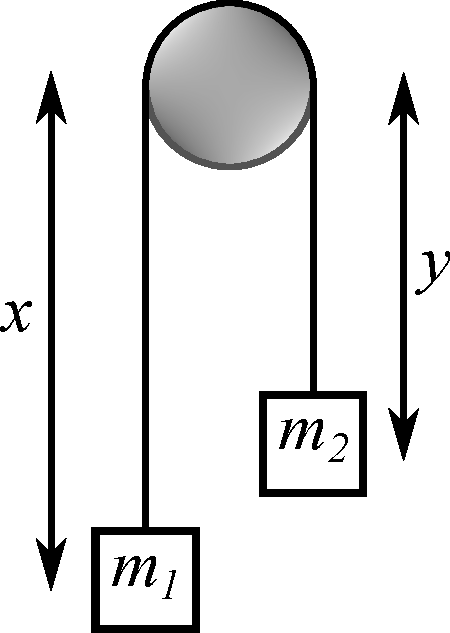
\includegraphics[width=.3\textwidth]{mekfigs/Atwood.pdf}
	\caption{Illustration af Atwoods faldmaskine, hvor to lod forbindes med en snor over en trisse.}
	\label{mek:fig:Atwood}
\end{figure}
%
%
\begin{opgave}[2]{Atwoods faldmaskine} \label{mek:opg:Atwood}%
I \cref{mek:fig:Atwood} ses en illustration af Atwoods faldmaskine, hvori to lodder hænges i hver sin ende af en snor med konstant længde $l$. I figuren er to koordinater også defineret, og de to lodders masser er indtegnet.
%
\opg Argumenter for at der kun er ét generaliseret koordinat.
%
\opg Udtryk $y$ ved $x$.
%
\opg Udtryk $\dot{y}$ ved $\dot{x}$.
%
\opg Definer hhv. $x = 0$ og $y = 0$ som nulpunkt for den potentielle energi for hvert lod, og opskriv den totale potentielle energi\footnote{Har man svært ved at acceptere gyldigheden af at regne med negativ potentiel energi, kan man godt definere nulpunktet under faldmaskinen, hvilket gør at Lagrangefunktionen kommer til at indeholde nogle ekstra konstanter.}.
%
\opg Opskriv den kinetiske energi som summen af den kinetiske energi for hver af de to lodder.
%
\opg Vis at Lagrangefunktionen for systemet kan skrives på formen
%
\begin{align*}
	L(x,\dot{x},t) = \frac{1}{2}(m_1+m_2)\dot{x}^2
	+ g\Big(m_1x + m_2(l-x-\pi R)\Big).
\end{align*}
%
\opg Vis ved brug af Euler-Lagrangeligningen, at systemets bevægelsesligning er
%
\begin{align} \label{mek:eq:atwood}
	\ddot{x} = g\frac{m_1-m_2}{m_1+m_2}.
\end{align}
%
\opg Argumentér for at højresiden af \cref{mek:eq:atwood} er en konstant.
%
\opg Slå løsningen til differentialligningen i \cref{mek:eq:atwood} op i \cref{k-mat:tab:diffligninger} i kompendiet.
%
\opg Beskriv lodernes bevægelse med ord og sammenlign med det frie fald uden luftmodstand. \textit{Hint}: se \cref{k-mat:ex:frit_fald} i \cref{k-chap:matematik} i kompendiet.
\end{opgave}
% Der er ingen grund til at gøre opgaven sværere end den allerede er. Differentialligningen løses ved tabelopslag i stedet for seperation af de variable som nedenfor.
% \opg Vis ud fra bevægelsesligningen, hvad fortegnet af $\ddot{x}$ er afhængigt af om $m_1>m_2$ eller $m_2>m_1$. Hvilket af de to lodder vil falde ned (hvad betyder det for retningen af bevægelsen)? \\ 
% %
% Skrives bevægelsesligningen lidt om fås
% %
% \begin{align*}
% 	\dv[2]{x}{t} = g\frac{m_1-m_2}{m_1+m_2} &= a \\
% 	\implies \dv{}{t}\left( \dv{x}{t} \right) &= a \\
% 	\implies \dv{x}{t} &= \int a \dd{t}\\
% 	\implies x(t) &= \int\int a \dd{t}\dd{t}
% \end{align*}
% %
% Det trick vi bruger her er, at integration og differentiation er hinandens omvendte operationer ligesom plus og minus er hinandens omvendte operationer.\footnote{Faktisk har vi også antaget, at to integrationskonstanter er $0$, men det er en mindre detalje.} 
% %
% \opg Bestem $x(t)$ ved ovenstående integral.\\ 
% \textit{Hint}: Regn det inderste integrale, så det yderste.


\begin{figure}[]
\centering
    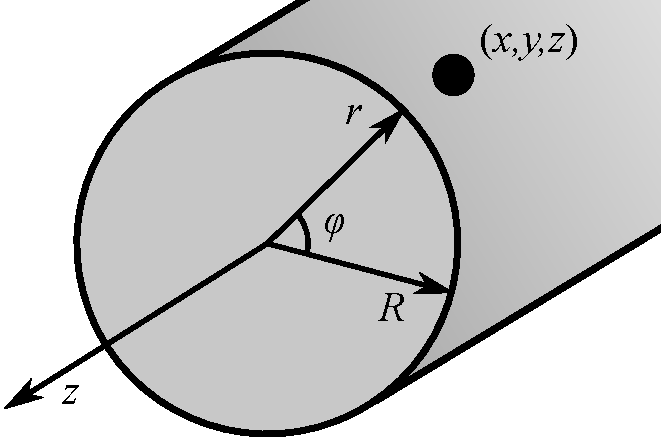
\includegraphics[width = .42\textwidth]{mekfigs/cylinderopg_sh.pdf}
    \caption{Partikel på cylinder. På figuren er både de kartesiske og cylindrisk polære koordinater indikeret.}
    \label{mek:fig:cyl}
\end{figure}
%
\begin{opgave}[2]{Partikel på en cylinder} \label{mek:opg:Cylinder}%
Vi ser på en partikel, der kan bevæge sig frit på overfladen af en cylinder med radius $R$, som det ses på \cref{mek:fig:cyl}. Her er det oplagt at bruge cylindriske koordinater:
%
\begin{align*}
x &= r\cos(\phi), \\
y &= r\sin(\phi), \\
z &= z.
\end{align*}
%
\opg Brug de cylindriske koordinater som generaliserede koordinater. Hvilke koordinater ændres, når partiklen bevæger sig?
%
\opg Udregn $\dot{x}$, $\dot{y}$ og $\dot{z}$ i de nye koordinater.
%
\opg Opstil den kinetiske energi, $K=\frac{1}{2}mv^2$.
%
\opg Opstil Lagrangefunktionen, hvor den potentielle energi er altid nul.
%
\opg Brug Euler-Lagrangeligningerne til at opstille andenordensdifferentialligninger for de koordinater, der ændres, når partiklen bevæger sig.
%
\opg Hvordan bevæger partiklen sig?
\end{opgave}

\begin{figure}[]
	\centering
	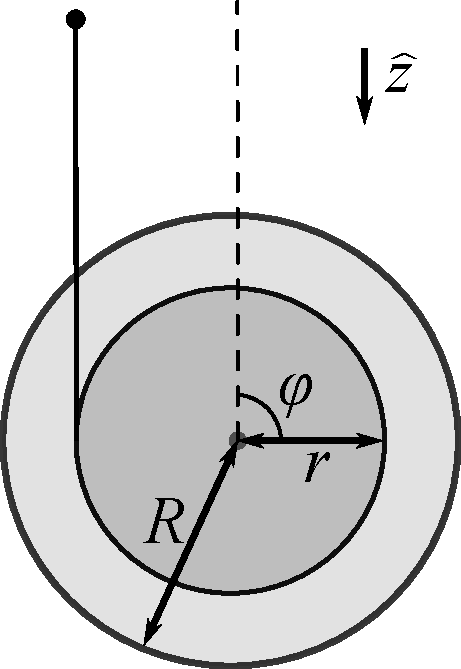
\includegraphics[width=.32\textwidth]{mekfigs/yoyo.pdf}
	\caption{Skitse af en simpel yoyomodel med radier $r$ og $R$ i et tyngdefelt med i nedadgående retning med styrken $g$.}
	\label{mek:fig:yoyo}
\end{figure}
%
\begin{opgave}[2]{Yoyo} \label{opg:Yoyo}%
Betragt yoyoen i \cref{mek:fig:yoyo} med massen $m$ og de fysiske dimensioner som vist i figuren.
% Da stive legemers rotation ikke er introduceret på campen, er inertimomentet ukendt, hvorfor Lagrangefunktionen gives.
Tyngdekraften har størrelsen $g$ i $z$-retningen, $\va{F}_\textup{g} = mg \vu{z}$, og den ideelle snor sidder fast i afstanden $r$ fra centrum. At snoren er ideel betyder, at den anses som ustrækkelig, masseløs, og derudover anses friktionen mellem snoren og yoyoen som værende så stor, at yoyoen ikke glider.
% Det kan vises, at yoyoens inertimoment i denne model er
% \begin{align*}
% 	I = \frac{1}{2}mR^2 \: .
% \end{align*}
% Som generaliseret koordinat benyttes $z$, fordi $z$ og $\phi$ er koblede.
% \opg 
Antagelsen at friktionen mellem snoren og yoyoen er tilpas stor, gør at det punkt hvor snoren slipper yoyoen står stille, hvilket betyder, at rotationen lige præcis udligner bevægelsen fra at hele yoyoen falder nedad\footnote{Dette kaldes ofte at yoyoen \textit{ruller uden at glide}, hvilket er en meget almindelig antagelse i fysik.}.
% Det betyder, at farten $v$ i ligning \eqref{k-eq:SmartFart} er lig med farten $v_\textsc{cm}$ i ligning \eqref{k-eq:K}, hvor begge ligninger henviser til kompendiet. Brug disse ligninger til at vise at
På baggrund af de antagelser kan man vise at yoyoens kinetiske energi er
%
\begin{align} \label{mek:eq:yoyo_kin}
	K = \frac{1}{2}m\dot{z}^2 + \frac{1}{4}mR^2\left(\frac{\dot{z}}{r}\right)^2.
\end{align}
%
Man behøver ikke forstå hvor \cref{mek:eq:yoyo_kin} kommer fra -- det kan tages for gode varer.
%
\opg Argumenter for at den potentielle energi kan skrives på formen $V = -mgz$.
%
\opg Konkluder at Lagrangefunktionen for situationen er
%
\begin{align*}
	L = \frac{1}{2}m\left[1 + \frac{1}{2}\left(\frac{R}{r}\right)^2\right]\dot{z}^2 + mgz.
\end{align*}
%
\opg Bestem nu følgende afledte af Lagrangefunktionen
%
\begin{align*}
	\pdv{L}{z} &= \; ? \\
	\pdv{L}{\dot{z}} &= \; ? \\
	\el{z} &= \; ?
\end{align*}
%
\opg Brug Euler-Lagrangeligningen, \cref{k-mek:eq:Euler-Lagrange} i kompendiet, til at vise at
%
\begin{align} \label{mek:eq:YoyoDiffLign}
	\ddot{z} = \frac{g}{1 + R^2/(2r^2)}.
\end{align} \\[1mm]
%
Løsningen til denne differentialligning kan ved hjælp af \cref{k-mat:tab:diffligninger} i kompendiet ses til at være
%
\begin{align} \label{mek:eq:YoyoBevLign}
	z(t) = \frac{g}{2}\left[1 + \frac{1}{2}\left(\frac{R}{r}\right)^2\right]^{-1}t^2 + v_0t + z_0,
\end{align}
%
hvor $v_0$ er startfarten, og $z_0$ er startstedkoordinatet. Ved indsættelse i \cref{mek:eq:YoyoDiffLign} kan det vises, at \cref{mek:eq:YoyoBevLign} er en løsning.
%
\opg Beskriv yoyoens bevægelse med ord og sammenlign med det frie fald uden luftmodstand. \textit{Hint}: se \cref{k-mat:ex:frit_fald} i \cref{k-chap:matematik} i kompendiet.
%
\opg Overvej hvilke fordele og ulemper der er, ved at benytte Lagrangemekanikken til at løse dette problem frem for Newtonsk mekanik.
\end{opgave}


\begin{opgave}[3]{Elektriske kredsløb og kvantecomputere}
%
\begin{wrapfigure}{r}{0.41\textwidth}
	\centering
	\ctikzset{bipoles/thickness=1}
	\begin{circuitikz}[line width=1.3pt, scale=1.5]
	    \coordinate (o) at (0,0);
	    %
		\draw (0,-0.2) node[ tlground, line width=.45pt ] {};
		\draw (0,-0.2) to [ short ](o) to [ short ] (-.75,0)
		to [ barrier ] (-.75,2) to [ short ] (0,2);
		\draw (o) to [ short ] (.75,0)
		to [ C, l_=$C$ ] (.75,2) to [ short ] (0,2);
		\draw (-.85,1) node[anchor=east]{$E_\textup{J}$};
		\fill (0,2) circle (0.75 mm);
	    \draw (0,2.05) node[anchor=south]{$\phi$};
		\fill (o) circle (0.75 mm);
	    \draw (0,0.05) node[anchor=south]{$g$};
	\end{circuitikz}
	\caption{Kredsløbsdiagram af en såkaldt transmon, der består en kondensator med kapacitans $C$ og en Josephsonkontakt med Josephsonenergi $E_\textup{J}$. Kredsløbets generaliserede koordinat er knudepunktsfluxen $\phi$, og kredsløbet er koblet til jord i knudepunktet $g$.}
	\label{mek:fig:transmon}
\end{wrapfigure}
%
\Cref{mek:fig:transmon} viser et kredsløbsdiagram for en såkaldt transmon, der er en nøglekomponent i moderne forskning om brugen af superledende kredsløb til kvantecomputere. Transmonen består af to komponenter: en kondensator med kapacitans $C$, og en såkaldt Josephsonkontakt med Josephsonenergi $E_\textup{J}$. Kredsløbet er beskrevet af Lagrangefunktionen
%
\begin{align} \label{mek:eq:transmon}
	L = \frac{1}{2}C\dot{\phi}^2 + E_\textup{J}\cos(\phi).
\end{align}
%
Det kræver kvantemekanik, at beskrive virkelige transmoner og forstå Josephsonkontakten, men derfor kan man stadig regne på, hvordan transmonen ville virke, hvis ikke det var nødvendigt med kvantemekanik.
%
\opg Brug Euler-Lagrangeligningen til at vise, at transmonens klassiske bevægelsesligning kan skrives på formen
%
\begin{align} \label{mek:eq:transmon_eom}
    \ddot{\phi} = -\omega\sin(\phi).
\end{align}
%
\opg Hvad er $\omega$ udtrykt ved $C$ og $E_\textup{J}$?
%
\opg Hvilket mekanisk system fra kompendiet er også beskrevet af bevægelsesligningen i \cref{mek:eq:transmon_eom}?
%
\opg Benyt samme approksimation som i kompendiet, til at vise at
%
\begin{align} \label{mek:eq:transmon_eom2}
    \ddot{\phi} \simeq -\omega\phi.
\end{align}
%
\opg Hvad skal gælde for at \cref{mek:eq:transmon_eom2} er en gyldig approksimation? \\%[1mm]

Hvis man vil bruge en transmon til en kvantecomputer, så viser det sig at være vigtigt, at \cref{mek:eq:transmon_eom2} ikke er en god approksimation. Mere specifikt vil man gerne have en såkaldt anharmonisk oscillator på formen
%
\begin{align} \label{mek:eq:transmon_eom3}
    \ddot{\phi} \simeq - \omega\phi + K_3\phi^3.
\end{align}
%
\opg Vis at \cref{mek:eq:transmon_eom3} også er en approksimation af \cref{mek:eq:transmon_eom} og bestem værdien af $K_3$.
%
\opg Hvad skal gælde om $\omega$ og $K_3$, for at \cref{mek:eq:transmon_eom3} er en god approksimation af \cref{mek:eq:transmon_eom}, samtidig med at \cref{mek:eq:transmon_eom2} er en dårlig approksimation?
\end{opgave}


% Denne opgave kan ikke løses, da stive legemers roterende bevægelse ikke er introduceret
% \begin{opgave}{Cylinder på skråplan}{2} \label{mek:opg:cylinder}
% En cylinder med massen $m$, radius $R$ og inertimoment $I$ placeres på et skråplan med vinklen $\alpha$ i forhold til vandret.\\
% \opg Skitser situationen.
% \opg Indtegn på skitsen det koordinatsystem, der giver det færrest mulige afhængige koordinater.
% \opg Opstil den potentielle energi $V$ for systemet, hvor der ses bort fra cylinderes udtrækning.
% \opg Udtryk den kinetiske energi $K$ ved cylinderens fysiske parametre og tidsafledede af de valgte generaliserede koordinater.
% \opg Opskriv problemets Lagrangefunktion.
% \opg Vis at ved løsning af Euler-Lagrangeligningen fåes
% \begin{align*}
% \ddot{x} = -\frac{g\sin\alpha}{1+I/mR^2} \: .
% \end{align*}
% \opg Argumenter for at accelerationen er konstant.
% \opg Lad nu accelerationen være $\tilde{g}$, og vis at bevægelsesligningens løsning er
% \begin{align*}
% x(t) = \frac{1}{2}\tilde{g}t^2 + v_0t + x_0 \: .
% \end{align*}
% \end{opgave}


\begin{figure}[t]
	\centering
	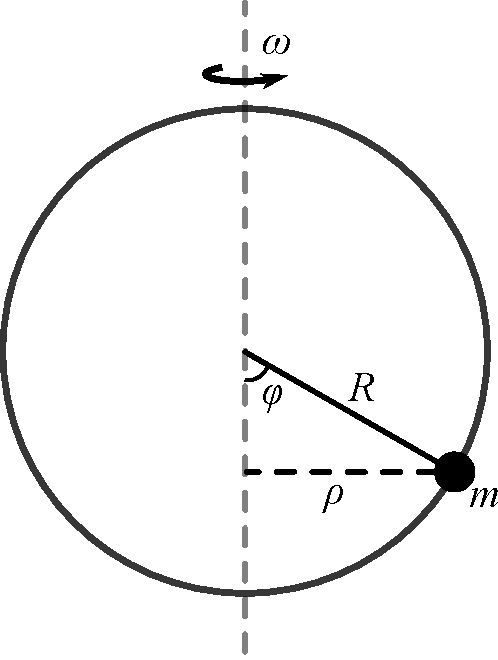
\includegraphics[width=.35\columnwidth]{mekfigs/BeadOnHoop.pdf}
	\caption{Illustration af situationen, hvor koordinater og andre parametre er indtegnet.} \label{mek:fig:BeadOnHoop}
\end{figure}
%
\begin{opgave}[3]{Masse på roterende ring}
Et lod med masse $m$ er placeret på en ring, hvorpå den kan bevæge sig friktionsløst, som i \cref{mek:fig:BeadOnHoop}. Ringen har radius $R$, og den roterer om sin egen akse med vinkelhastigheden $\omega$. Massen kan beskrives udelukkende ved det generaliserede koordinat $\phi$, men for at indse dette gøres brug af koordinatet $\rho$.
%
\opg Udtryk den potentielle energi ved det generaliserede koordinat $\phi$, således at $V(\phi=0)=0$. \textit{Hint}: se \cref{k-mek:ex:PendulLagrange} i \cref{k-chap:mek} i kompendiet.
%
\opg Massens hastighed deles nu op i to komposanter -- en der svarer til ind i tegningen og en langs ringen. Disse kaldes henholdsvis $v_\textup{ring}$, idet det er bevægelsen som følge af ringens rotation, og $v_\textup{lod}$ idet det er lodets bevægelse på ringen. Bestem disse komposanter udtrykt ved $\omega$, $\phi$ og $\dot{\phi}$, samt eventuelle geometriske parametre. \textit{Hint}: Benyt \cref{k-mek:eq:SmartFart} i kompendiet.
%
\opg Brug dette til at bestemme den kinetiske energi, og vis dermed at Lagrangefunktionen er
%
\begin{align*}
	L = \frac{1}{2}mR^2\big[\dot{\phi}^2 + \omega^2\sin^2(\phi)\big] - mgR\big[1-\cos(\phi)\big].
\end{align*}
%
\opg Benyt Euler-Lagrangeligningen til at vise, at bevægelsesligningen er
%
\begin{align*}
	\ddot{\phi} = \left[\omega^2\cos(\phi) - \frac{g}{R}\right]\sin(\phi).
\end{align*}
%
\opg Hvad er kriteriet for henholdsvis et stabilt og ustabilt ligevægtspunkt fysisk og matematisk?
%
\opg Brug kriterierne til at bestemme systemets ligevægtspunkter, og forklar hvad de betyder fysisk.
%
\opg Eksister alle disse punkter for alle værdier af $\omega, R$ og $g$?
%
\opg Diskuter om ligevægtspunkterne er stabile eller ustabile i alle tilfælde fra sidste spørgsmål.%\footnote{Ligevægtspunkterne $\phi_0 = 0,\pm\pi$ er ikke super komplicerede at vise stabiliteten af matematisk, men det sidste er svært, hvorfor dette bør tilgås med forsigtighed. Det er dog vist i facitlisten, hvordan dette gøres, hvilket kan være en gennemlæsning værd.}.
\end{opgave}

\section*{Flerlegemeproblemer}


\begin{figure}[]
    \centering
    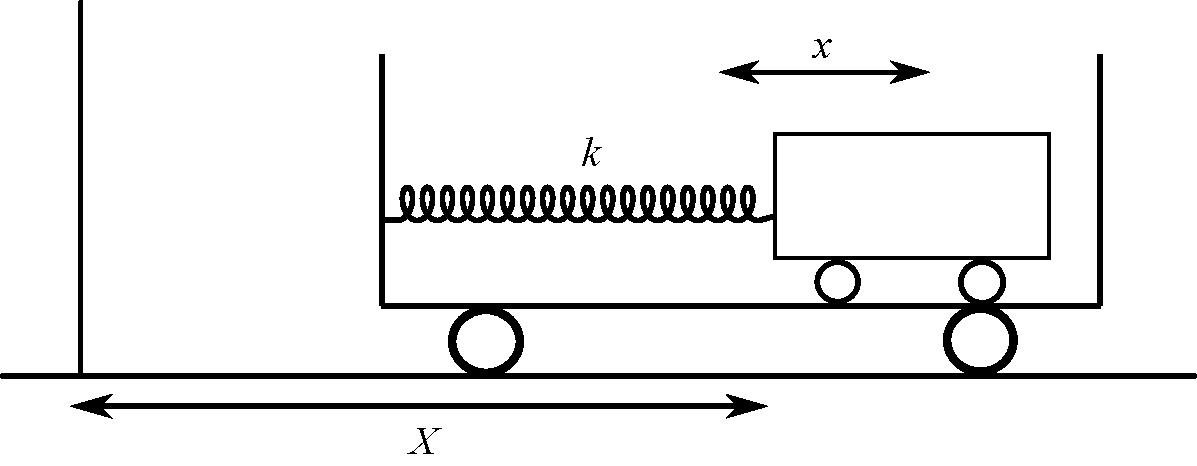
\includegraphics[width=.65\textwidth]{mekfigs/ToKobledeVogne.pdf}
    \caption{Illustration af situationen i \cref{mek:opg:ToKobledeVogne}. $X$ er stedkoordinatet for den store vogn, og $x$ er stedkoordinatet for den lille, hvor $x=0$ defineres som midtpunktet i den store vogn. Fjederens fjederkonstant kaldes $k$ som sædvanligt.}
    \label{mek:fig:ToKobledeVogne}
\end{figure}
%
\begin{opgave}[2]{To koblede vogne} \label{mek:opg:ToKobledeVogne}%
En lille vogn med massen $m$ placeres i en større vogn, og de to forbindes med en fjeder med fjederkonstant $k$. Den lille vogn antages at kunne bevæge sig friktionsløst i forhold til den store og den store i forhold til underlaget, og de generaliserede koordinater defineres som på \cref{mek:fig:ToKobledeVogne}. Den store vogn tvinges til simpel harmonisk bevægelse, det vil sige $X = A\cos(\omega t)$, hvor $A,\omega$ er konstanter, og derudover kaldes den lille vogns naturlige vinkelfrekvens $\omega_0 = \sqrt{k/m}$.
%
\opg Argumenter for at den lille vogns hastighed i forhold til underlaget kan skrives som
%
\begin{align*}
    v = \dot{x} + \dot{X},
\end{align*}
%
og brug dette til at indse, at
%
\begin{align*}
    K = \frac{1}{2}m\left(\dot{x} + \dot{X}\right)^2.
\end{align*}
%
\opg Argumenter for at den potentielle energi for den lille vogn er
%
\begin{align*}
    V = \frac{1}{2}kx^2,
\end{align*}
%
og konkluder at
%
\begin{align*}
    L = \frac{1}{2}m\left(\dot{x} + \dot{X}\right)^2 - \frac{1}{2}kx^2.
\end{align*}
%
\opg Brug dette til at vise, at
%
\begin{align*}
    \pdv{L}{\dot{x}} &= m(\dot{x} + \dot{X}), \\
    \pdv{L}{x} &= -kx.
\end{align*}
%
\opg Vis at
%
\begin{align*}
    \el{x} = m\ddot{x} - Am\omega^2\cos(\omega t),
\end{align*}
%
og konkluder at
%
\begin{align*}
    \ddot{x} + \frac{k}{m}x = A\omega^2\cos(\omega t).
\end{align*}
%
\opg Fastholdes den store vogn nu i $X=0$ bliver systemet i denne opgave ækvivalent til et system, uden den store vogn, hvor fjederen på den lille vogn er spændt fast på væggen, hvilket er en harmonisk oscillator. $X=0$ kan realiseres ved at sætte $A=0$. Vis at bevægelsesligningen i dette tilfælde reducerer til en harmonisk oscillator.
%
\opg Hvorfor er det relevant at tjekke, at systemet reducerer til en harmonisk oscillator i grænsen $A=0$?
\end{opgave}


\begin{figure}[]
\centering
    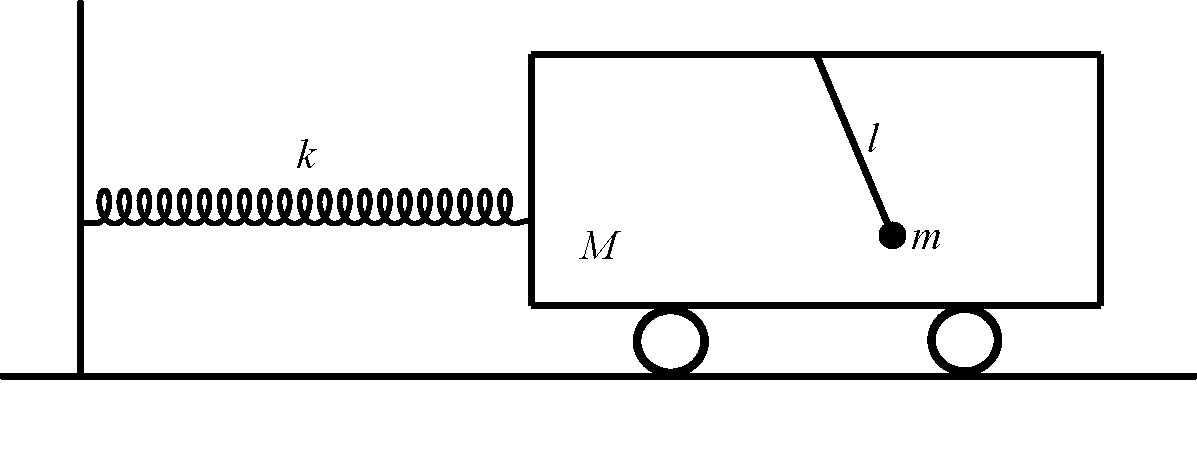
\includegraphics[width=0.65\textwidth]{mekfigs/PendulIVognOpg.pdf}
    \caption{Pendul med massen $m$ og længden $l$ placeret i en vogn med massen $M$, der er fastgjort til en væg med en en fjeder med fjederkonstant $k$.}
    \label{mek:fig:PendulIVognOpg}
\end{figure} 
%
\begin{opgave}[4]{Pendul i en vogn}
I \cref{mek:fig:PendulIVognOpg} er der tegnet et pendul, ophængt i en vogn, der tilmed er fastspændt med en fjeder til en væg, og de relevante fysiske størrelser er indtegnet.
%
\opg Identificer systemets generaliserede koordinater, indtegn enhedsvektorerne for et kartesisk koordinatsystem og definer origo. %(hint: Se beskrivelsen af pendulet med Lagrangeformalismen og opgave \ref{opg:ToKobledeVogne})
%
\opg Opskriv pendulets kartesiske koordinater, $(X_p,Y_p)$, udtrykt ved de generaliserede koordinater, samt vognens kartesiske $X$-koordinat, $X_v$, og argumenter for, at $Y_v$ er ubetydelig for problemet.
%
\opg Bestem systemets potentielle energi.
%
\opg Bestem systemets kinetiske energi og opskriv Lagrangefunktionen. %(hint: Anvend de kartesiske koordinater fra sidste opgave til først at bestemme de relevante hastigheder)
%
\opg Vis at løsningen til Euler-Lagrangeligningen er de koblede differentialligninger
%
\begin{align*}
    a&) \quad M\ddot{x} + m\ddot{x} + ml\ddot{\phi}\cos\phi - ml\dot{\phi}^2\sin\phi = -kx, \\
    b&) \quad ml^2\ddot{\phi} + ml\ddot{x}\cos\phi = -mgl\sin\phi,
\end{align*}
%
hvis de generaliserede koordinater vælges til at være vognes placering, $x$, og pendulets udsvingsvinkel $\phi$.
%
\opg Bestem Taylorudviklingen til 1. orden i $\phi$ af bevægelsesligningerne. \\ \\
Nu kigges på grænserne
%
\begin{enumerate}
    \item $k \rightarrow \infty$,
    \item $M \gg m$.
\end{enumerate}
%
\opg Hvilken fysisk situation svarer hver grænse til?
%
\opg Hvad forventes systemet at blive til i de ovenstående grænser?
%
\opg Hvad bliver det til?
\end{opgave}
%
\end{document}